% Options for packages loaded elsewhere
\PassOptionsToPackage{unicode}{hyperref}
\PassOptionsToPackage{hyphens}{url}
%
\documentclass[
  english,
  man]{apa6}
\usepackage{amsmath,amssymb}
\usepackage{lmodern}
\usepackage{ifxetex,ifluatex}
\ifnum 0\ifxetex 1\fi\ifluatex 1\fi=0 % if pdftex
  \usepackage[T1]{fontenc}
  \usepackage[utf8]{inputenc}
  \usepackage{textcomp} % provide euro and other symbols
\else % if luatex or xetex
  \usepackage{unicode-math}
  \defaultfontfeatures{Scale=MatchLowercase}
  \defaultfontfeatures[\rmfamily]{Ligatures=TeX,Scale=1}
\fi
% Use upquote if available, for straight quotes in verbatim environments
\IfFileExists{upquote.sty}{\usepackage{upquote}}{}
\IfFileExists{microtype.sty}{% use microtype if available
  \usepackage[]{microtype}
  \UseMicrotypeSet[protrusion]{basicmath} % disable protrusion for tt fonts
}{}
\makeatletter
\@ifundefined{KOMAClassName}{% if non-KOMA class
  \IfFileExists{parskip.sty}{%
    \usepackage{parskip}
  }{% else
    \setlength{\parindent}{0pt}
    \setlength{\parskip}{6pt plus 2pt minus 1pt}}
}{% if KOMA class
  \KOMAoptions{parskip=half}}
\makeatother
\usepackage{xcolor}
\IfFileExists{xurl.sty}{\usepackage{xurl}}{} % add URL line breaks if available
\IfFileExists{bookmark.sty}{\usepackage{bookmark}}{\usepackage{hyperref}}
\hypersetup{
  pdftitle={Measurement Invariance of the Dirty Dozen: Student and Working Adult Samples},
  pdfauthor={Yang Yang1 \& John Kulas2},
  pdflang={en-EN},
  pdfkeywords={keywords},
  hidelinks,
  pdfcreator={LaTeX via pandoc}}
\urlstyle{same} % disable monospaced font for URLs
\usepackage{graphicx}
\makeatletter
\def\maxwidth{\ifdim\Gin@nat@width>\linewidth\linewidth\else\Gin@nat@width\fi}
\def\maxheight{\ifdim\Gin@nat@height>\textheight\textheight\else\Gin@nat@height\fi}
\makeatother
% Scale images if necessary, so that they will not overflow the page
% margins by default, and it is still possible to overwrite the defaults
% using explicit options in \includegraphics[width, height, ...]{}
\setkeys{Gin}{width=\maxwidth,height=\maxheight,keepaspectratio}
% Set default figure placement to htbp
\makeatletter
\def\fps@figure{htbp}
\makeatother
\setlength{\emergencystretch}{3em} % prevent overfull lines
\providecommand{\tightlist}{%
  \setlength{\itemsep}{0pt}\setlength{\parskip}{0pt}}
\setcounter{secnumdepth}{-\maxdimen} % remove section numbering
% Make \paragraph and \subparagraph free-standing
\ifx\paragraph\undefined\else
  \let\oldparagraph\paragraph
  \renewcommand{\paragraph}[1]{\oldparagraph{#1}\mbox{}}
\fi
\ifx\subparagraph\undefined\else
  \let\oldsubparagraph\subparagraph
  \renewcommand{\subparagraph}[1]{\oldsubparagraph{#1}\mbox{}}
\fi
% Manuscript styling
\usepackage{upgreek}
\captionsetup{font=singlespacing,justification=justified}

% Table formatting
\usepackage{longtable}
\usepackage{lscape}
% \usepackage[counterclockwise]{rotating}   % Landscape page setup for large tables
\usepackage{multirow}		% Table styling
\usepackage{tabularx}		% Control Column width
\usepackage[flushleft]{threeparttable}	% Allows for three part tables with a specified notes section
\usepackage{threeparttablex}            % Lets threeparttable work with longtable

% Create new environments so endfloat can handle them
% \newenvironment{ltable}
%   {\begin{landscape}\centering\begin{threeparttable}}
%   {\end{threeparttable}\end{landscape}}
\newenvironment{lltable}{\begin{landscape}\centering\begin{ThreePartTable}}{\end{ThreePartTable}\end{landscape}}

% Enables adjusting longtable caption width to table width
% Solution found at http://golatex.de/longtable-mit-caption-so-breit-wie-die-tabelle-t15767.html
\makeatletter
\newcommand\LastLTentrywidth{1em}
\newlength\longtablewidth
\setlength{\longtablewidth}{1in}
\newcommand{\getlongtablewidth}{\begingroup \ifcsname LT@\roman{LT@tables}\endcsname \global\longtablewidth=0pt \renewcommand{\LT@entry}[2]{\global\advance\longtablewidth by ##2\relax\gdef\LastLTentrywidth{##2}}\@nameuse{LT@\roman{LT@tables}} \fi \endgroup}

% \setlength{\parindent}{0.5in}
% \setlength{\parskip}{0pt plus 0pt minus 0pt}

% \usepackage{etoolbox}
\makeatletter
\patchcmd{\HyOrg@maketitle}
  {\section{\normalfont\normalsize\abstractname}}
  {\section*{\normalfont\normalsize\abstractname}}
  {}{\typeout{Failed to patch abstract.}}
\patchcmd{\HyOrg@maketitle}
  {\section{\protect\normalfont{\@title}}}
  {\section*{\protect\normalfont{\@title}}}
  {}{\typeout{Failed to patch title.}}
\makeatother
\shorttitle{Measurement Invariance}
\keywords{keywords\newline\indent Word count: X}
\DeclareDelayedFloatFlavor{ThreePartTable}{table}
\DeclareDelayedFloatFlavor{lltable}{table}
\DeclareDelayedFloatFlavor*{longtable}{table}
\makeatletter
\renewcommand{\efloat@iwrite}[1]{\immediate\expandafter\protected@write\csname efloat@post#1\endcsname{}}
\makeatother
\usepackage{lineno}

\linenumbers
\usepackage{csquotes}
\ifxetex
  % Load polyglossia as late as possible: uses bidi with RTL langages (e.g. Hebrew, Arabic)
  \usepackage{polyglossia}
  \setmainlanguage[]{english}
\else
  \usepackage[main=english]{babel}
% get rid of language-specific shorthands (see #6817):
\let\LanguageShortHands\languageshorthands
\def\languageshorthands#1{}
\fi
\ifluatex
  \usepackage{selnolig}  % disable illegal ligatures
\fi
\newlength{\cslhangindent}
\setlength{\cslhangindent}{1.5em}
\newlength{\csllabelwidth}
\setlength{\csllabelwidth}{3em}
\newenvironment{CSLReferences}[2] % #1 hanging-ident, #2 entry spacing
 {% don't indent paragraphs
  \setlength{\parindent}{0pt}
  % turn on hanging indent if param 1 is 1
  \ifodd #1 \everypar{\setlength{\hangindent}{\cslhangindent}}\ignorespaces\fi
  % set entry spacing
  \ifnum #2 > 0
  \setlength{\parskip}{#2\baselineskip}
  \fi
 }%
 {}
\usepackage{calc}
\newcommand{\CSLBlock}[1]{#1\hfill\break}
\newcommand{\CSLLeftMargin}[1]{\parbox[t]{\csllabelwidth}{#1}}
\newcommand{\CSLRightInline}[1]{\parbox[t]{\linewidth - \csllabelwidth}{#1}\break}
\newcommand{\CSLIndent}[1]{\hspace{\cslhangindent}#1}

\title{Measurement Invariance of the Dirty Dozen: Student and Working Adult Samples}
\author{Yang Yang\textsuperscript{1} \& John Kulas\textsuperscript{2}}
\date{}


\authornote{

Add complete departmental affiliations for each author here. Each new line herein must be indented, like this line.

Enter author note here.

Correspondence concerning this article should be addressed to Yang Yang, Shanghai, China. E-mail: \href{mailto:yangyangsh@outlook.com}{\nolinkurl{yangyangsh@outlook.com}}

}

\affiliation{\vspace{0.5cm}\textsuperscript{1} Roche\\\textsuperscript{2} Montclair State University}

\abstract{
Now we are evaluating the psychometric properties of the dirty dozen simplified Chinese version by using samples in real settings: job applicants and incumbents (in addition to students). We replicate a previous study using the student sample, then continue to evaluate with organizational data. We find that the scales are non-invariant. Seems to be revisiting these articles: Geng, Sun, Huang, Zhu, and Han (2015) and Grigoras, Butucescu, Miulescu, Opariuc-Dan, and Iliescu (2020)
}



\begin{document}
\maketitle

Initially we were interested in looking at reliance on student samples. Now we are evaluating the psychometric properties of the dirty dozen (DD) simplified Chinese version by using samples in real settings: job applicants and incumbents (in addition to students). We replicate a previous study using the student sample (Yang gonna send some articles), then continue to evaluate with organizational data. We find that the scales are non-invariant.

SDSME another version (27 items).

All studies investigating psychometric properties of these scales use University students.

Some groups may be expected to exhibit different item-construct associations due to shifting motivational forces.

ITC guidlines for translating and adapting tests recommends looking at possible differences across motives (Commission, 2017). For example,

Yang's references: Church et al. (2011), Schoot, Lugtig, and Hox (2012), Schmitt and Kuljanin (2008), Geng, Sun, Huang, Zhu, and Han (2015), Grigoras, Butucescu, Miulescu, Opariuc-Dan, and Iliescu (2020), Jonason and Webster (2010)

\hypertarget{methods}{%
\section{Methods}\label{methods}}

We follow the We also look at intercorrelations among items within the samplings.

\hypertarget{participants}{%
\subsection{Participants}\label{participants}}

In total 1106 individuals responded to the Dirty Dozen (as well as additional scales not the focus of the current presentation). This total was comprised of 208 working adults low-stakes, 527 working adults high-stakes, and 371 students low-stakes individuals. After screening for undifferentiated responses via the \texttt{R} package \texttt{careless} (Yentes \& Wilhelm, 2021), we retained 1054 respondents who had no more than 6 sequentially identical responses across the 12 total items.

\hypertarget{material}{%
\subsection{Material}\label{material}}

\hypertarget{procedure}{%
\subsection{Procedure}\label{procedure}}

Decrease in \(\Delta\chi^2\) across models indicates a lack of invariance (typically not considered a ``good thing''). Multiple indices are consulted across models, including \(\Delta\chi^2\), RMSEA, CFI, TLI, BIC, and AIC.

Also want to look at correlations of the simplified Chinese version of the DD with the Honesty-Humility subscales (Sincerity, Fairness, Greed Avoidance, and Modesty).

\hypertarget{data-analysis}{%
\subsection{Data analysis}\label{data-analysis}}

We used R {[}Version 4.0.5; R Core Team (2021){]} and the R-packages \emph{careless} {[}Version 1.2.1; Yentes and Wilhelm (2021){]}, \emph{corx} {[}Version 1.0.6.1; Conigrave (2020){]}, \emph{foreign} {[}Version 0.8.81; R Core Team (2020){]}, \emph{lavaan} {[}Version 0.6.8; Rosseel (2012){]}, \emph{papaja} {[}Version 0.1.0.9997; Aust and Barth (2020){]}, and \emph{semTools} {[}Version 0.5.5; Jorgensen, Pornprasertmanit, Schoemann, and Rosseel (2021){]} for all our analyses.

\begin{figure}
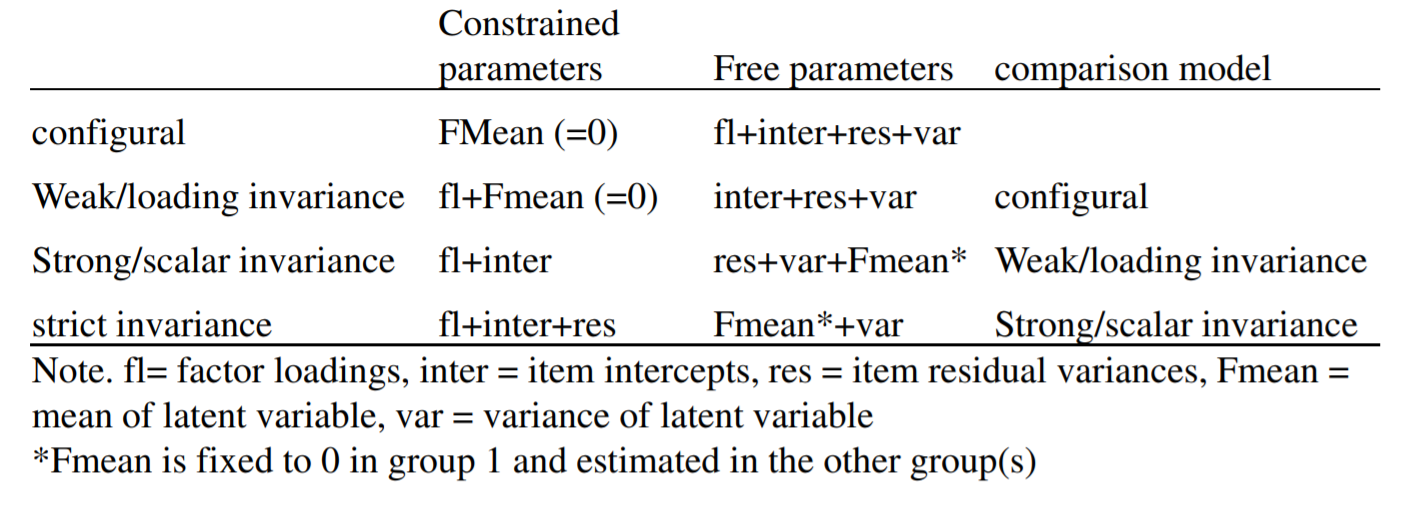
\includegraphics[width=4.71in]{steps} \caption{Steps for measurement invariance (taken from Xu, 2012).}\label{fig:figure1}
\end{figure}

\hypertarget{results}{%
\section{Results}\label{results}}

We looked at structural invariance as well as latent means (Meredith, 1993; Steinmetz, Schmidt, Tina-Booh, Wieczorek, \& Schwartz, 2009). The models failed to exhibit metric invariance (Model 2 - Model 1 exhibited a significant \(\Delta\) on both \(\chi^2\) as well as RMSEA)

\begin{quote}
Not sure how to pull table or identify object elements - \texttt{model1} object is too large to navigate easily.
\end{quote}

\begin{verbatim}
## 
## Measurement invariance models:
## 
## Model 1 : fit.configural
## Model 2 : fit.loadings
## Model 3 : fit.intercepts
## Model 4 : fit.means
## 
## Chi-Squared Difference Test
## 
##                 Df   AIC   BIC  Chisq Chisq diff Df diff Pr(>Chisq)    
## fit.configural 153 37059 37640 1407.7                                  
## fit.loadings   171 37135 37626 1518.9     111.25      18  1.837e-15 ***
## fit.intercepts 189 37230 37632 1650.5     131.54      18  < 2.2e-16 ***
## fit.means      195 37344 37716 1775.9     125.40       6  < 2.2e-16 ***
## ---
## Signif. codes:  0 '***' 0.001 '**' 0.01 '*' 0.05 '.' 0.1 ' ' 1
## 
## 
## Fit measures:
## 
##                  cfi rmsea cfi.delta rmsea.delta
## fit.configural 0.641 0.153        NA          NA
## fit.loadings   0.615 0.150     0.027       0.003
## fit.intercepts 0.582 0.148     0.032       0.001
## fit.means      0.548 0.152     0.034       0.004
\end{verbatim}

\begin{verbatim}
## lavaan 0.6-8 ended normally after 108 iterations
## 
##   Estimator                                         ML
##   Optimization method                           NLMINB
##   Number of model parameters                       117
##                                                       
##   Number of observations per group:                   
##     working adults low-stakes                      191
##     working adults high-stakes                     510
##     students low-stakes                            351
##                                                       
## Model Test User Model:
##                                                       
##   Test statistic                              1407.674
##   Degrees of freedom                               153
##   P-value (Chi-square)                           0.000
##   Test statistic for each group:
##     working adults low-stakes                  182.467
##     working adults high-stakes                 523.812
##     students low-stakes                        701.395
## 
## Model Test Baseline Model:
## 
##   Test statistic                              3696.466
##   Degrees of freedom                               198
##   P-value                                        0.000
## 
## User Model versus Baseline Model:
## 
##   Comparative Fit Index (CFI)                    0.641
##   Tucker-Lewis Index (TLI)                       0.536
## 
## Loglikelihood and Information Criteria:
## 
##   Loglikelihood user model (H0)             -18412.727
##   Loglikelihood unrestricted model (H1)     -17708.890
##                                                       
##   Akaike (AIC)                               37059.454
##   Bayesian (BIC)                             37639.593
##   Sample-size adjusted Bayesian (BIC)        37267.983
## 
## Root Mean Square Error of Approximation:
## 
##   RMSEA                                          0.153
##   90 Percent confidence interval - lower         0.146
##   90 Percent confidence interval - upper         0.160
##   P-value RMSEA <= 0.05                          0.000
## 
## Standardized Root Mean Square Residual:
## 
##   SRMR                                           0.110
## 
## Parameter Estimates:
## 
##   Standard errors                             Standard
##   Information                                 Expected
##   Information saturated (h1) model          Structured
## 
## 
## Group 1 [working adults low-stakes]:
## 
## Latent Variables:
##                    Estimate  Std.Err  z-value  P(>|z|)
##   mach =~                                             
##     A30               1.000                           
##     A31               0.392    0.095    4.111    0.000
##     A32               0.224    0.096    2.332    0.020
##     A33               0.538    0.063    8.507    0.000
##   narc =~                                             
##     A34               1.000                           
##     A35               0.262    0.263    0.996    0.319
##     A36               1.982    0.367    5.394    0.000
##     A37               1.752    0.332    5.277    0.000
##   psyc =~                                             
##     A38               1.000                           
##     A39               1.328    0.240    5.541    0.000
##     A40               0.820    0.195    4.196    0.000
##     A41               0.814    0.205    3.969    0.000
## 
## Covariances:
##                    Estimate  Std.Err  z-value  P(>|z|)
##   mach ~~                                             
##     narc              0.311    0.066    4.691    0.000
##     psyc              0.700    0.144    4.859    0.000
##   narc ~~                                             
##     psyc              0.251    0.065    3.863    0.000
## 
## Intercepts:
##                    Estimate  Std.Err  z-value  P(>|z|)
##    .A30               1.948    0.089   21.789    0.000
##    .A31               1.901    0.083   22.999    0.000
##    .A32               4.607    0.083   55.484    0.000
##    .A33               1.340    0.056   24.095    0.000
##    .A34               1.393    0.061   22.680    0.000
##    .A35               4.267    0.091   46.791    0.000
##    .A36               1.890    0.083   22.892    0.000
##    .A37               1.508    0.078   19.429    0.000
##    .A38               2.984    0.122   24.507    0.000
##    .A39               1.759    0.087   20.119    0.000
##    .A40               2.031    0.100   20.231    0.000
##    .A41               3.288    0.109   30.174    0.000
##     mach              0.000                           
##     narc              0.000                           
##     psyc              0.000                           
## 
## Variances:
##                    Estimate  Std.Err  z-value  P(>|z|)
##    .A30               0.678    0.099    6.865    0.000
##    .A31               1.174    0.122    9.608    0.000
##    .A32               1.274    0.131    9.725    0.000
##    .A33               0.345    0.041    8.401    0.000
##    .A34               0.562    0.063    8.951    0.000
##    .A35               1.578    0.162    9.753    0.000
##    .A36               0.682    0.099    6.890    0.000
##    .A37               0.666    0.088    7.523    0.000
##    .A38               2.350    0.247    9.509    0.000
##    .A39               0.610    0.098    6.251    0.000
##    .A40               1.601    0.168    9.514    0.000
##    .A41               1.948    0.204    9.572    0.000
##     mach              0.848    0.157    5.419    0.000
##     narc              0.158    0.052    3.008    0.003
##     psyc              0.482    0.172    2.812    0.005
## 
## 
## Group 2 [working adults high-stakes]:
## 
## Latent Variables:
##                    Estimate  Std.Err  z-value  P(>|z|)
##   mach =~                                             
##     A30               1.000                           
##     A31               0.495    0.059    8.361    0.000
##     A32               0.152    0.060    2.537    0.011
##     A33               0.398    0.031   12.716    0.000
##   narc =~                                             
##     A34               1.000                           
##     A35               0.377    0.148    2.544    0.011
##     A36               1.683    0.188    8.946    0.000
##     A37               0.622    0.098    6.323    0.000
##   psyc =~                                             
##     A38               1.000                           
##     A39               1.148    0.139    8.287    0.000
##     A40               0.408    0.087    4.692    0.000
##     A41               0.864    0.142    6.100    0.000
## 
## Covariances:
##                    Estimate  Std.Err  z-value  P(>|z|)
##   mach ~~                                             
##     narc              0.336    0.038    8.881    0.000
##     psyc              0.579    0.079    7.293    0.000
##   narc ~~                                             
##     psyc              0.251    0.039    6.388    0.000
## 
## Intercepts:
##                    Estimate  Std.Err  z-value  P(>|z|)
##    .A30               1.761    0.050   34.986    0.000
##    .A31               1.727    0.047   36.930    0.000
##    .A32               4.788    0.047  101.300    0.000
##    .A33               1.204    0.025   48.421    0.000
##    .A34               1.224    0.033   36.737    0.000
##    .A35               4.422    0.050   87.885    0.000
##    .A36               1.825    0.050   36.532    0.000
##    .A37               1.198    0.030   39.522    0.000
##    .A38               3.076    0.075   40.922    0.000
##    .A39               1.539    0.044   35.365    0.000
##    .A40               1.557    0.048   32.693    0.000
##    .A41               2.800    0.069   40.364    0.000
##     mach              0.000                           
##     narc              0.000                           
##     psyc              0.000                           
## 
## Variances:
##                    Estimate  Std.Err  z-value  P(>|z|)
##    .A30               0.564    0.053   10.564    0.000
##    .A31               0.938    0.061   15.403    0.000
##    .A32               1.123    0.070   15.926    0.000
##    .A33               0.200    0.014   14.029    0.000
##    .A34               0.434    0.030   14.306    0.000
##    .A35               1.272    0.080   15.941    0.000
##    .A36               0.902    0.068   13.291    0.000
##    .A37               0.418    0.027   15.564    0.000
##    .A38               2.415    0.158   15.304    0.000
##    .A39               0.350    0.048    7.324    0.000
##    .A40               1.079    0.069   15.726    0.000
##    .A41               2.105    0.137   15.401    0.000
##     mach              0.728    0.083    8.767    0.000
##     narc              0.131    0.026    4.974    0.000
##     psyc              0.468    0.108    4.315    0.000
## 
## 
## Group 3 [students low-stakes]:
## 
## Latent Variables:
##                    Estimate  Std.Err  z-value  P(>|z|)
##   mach =~                                             
##     A30               1.000                           
##     A31               0.322    0.076    4.220    0.000
##     A32               0.424    0.063    6.764    0.000
##     A33               0.854    0.078   10.963    0.000
##   narc =~                                             
##     A34               1.000                           
##     A35               1.286    0.240    5.359    0.000
##     A36               1.756    0.300    5.853    0.000
##     A37               1.486    0.276    5.387    0.000
##   psyc =~                                             
##     A38               1.000                           
##     A39               1.430    0.150    9.551    0.000
##     A40               0.785    0.119    6.627    0.000
##     A41               1.130    0.140    8.083    0.000
## 
## Covariances:
##                    Estimate  Std.Err  z-value  P(>|z|)
##   mach ~~                                             
##     narc              0.433    0.076    5.678    0.000
##     psyc              0.794    0.105    7.585    0.000
##   narc ~~                                             
##     psyc              0.326    0.060    5.403    0.000
## 
## Intercepts:
##                    Estimate  Std.Err  z-value  P(>|z|)
##    .A30               2.627    0.082   31.924    0.000
##    .A31               2.316    0.072   32.342    0.000
##    .A32               4.826    0.057   84.238    0.000
##    .A33               1.801    0.066   27.348    0.000
##    .A34               1.638    0.063   26.055    0.000
##    .A35               4.490    0.063   70.785    0.000
##    .A36               2.083    0.067   30.984    0.000
##    .A37               1.892    0.072   26.127    0.000
##    .A38               3.903    0.073   53.138    0.000
##    .A39               2.205    0.074   29.698    0.000
##    .A40               1.829    0.072   25.382    0.000
##    .A41               3.903    0.078   49.869    0.000
##     mach              0.000                           
##     narc              0.000                           
##     psyc              0.000                           
## 
## Variances:
##                    Estimate  Std.Err  z-value  P(>|z|)
##    .A30               1.474    0.124   11.919    0.000
##    .A31               1.707    0.129   13.240    0.000
##    .A32               0.990    0.075   13.148    0.000
##    .A33               0.863    0.076   11.335    0.000
##    .A34               1.276    0.095   13.396    0.000
##    .A35               1.227    0.093   13.238    0.000
##    .A36               1.241    0.099   12.522    0.000
##    .A37               1.593    0.120   13.220    0.000
##    .A38               1.407    0.109   12.936    0.000
##    .A39               0.938    0.085   11.028    0.000
##    .A40               1.522    0.116   13.139    0.000
##    .A41               1.528    0.119   12.827    0.000
##     mach              0.903    0.151    5.989    0.000
##     narc              0.112    0.039    2.896    0.004
##     psyc              0.487    0.099    4.944    0.000
\end{verbatim}

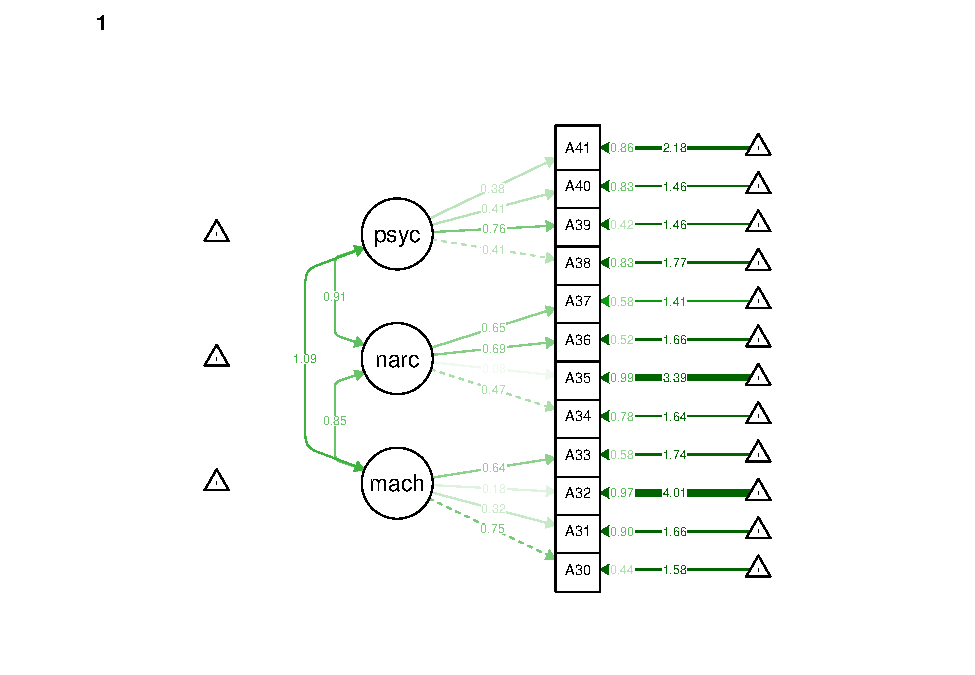
\includegraphics{SIOPpaper_files/figure-latex/measinv-1.pdf} 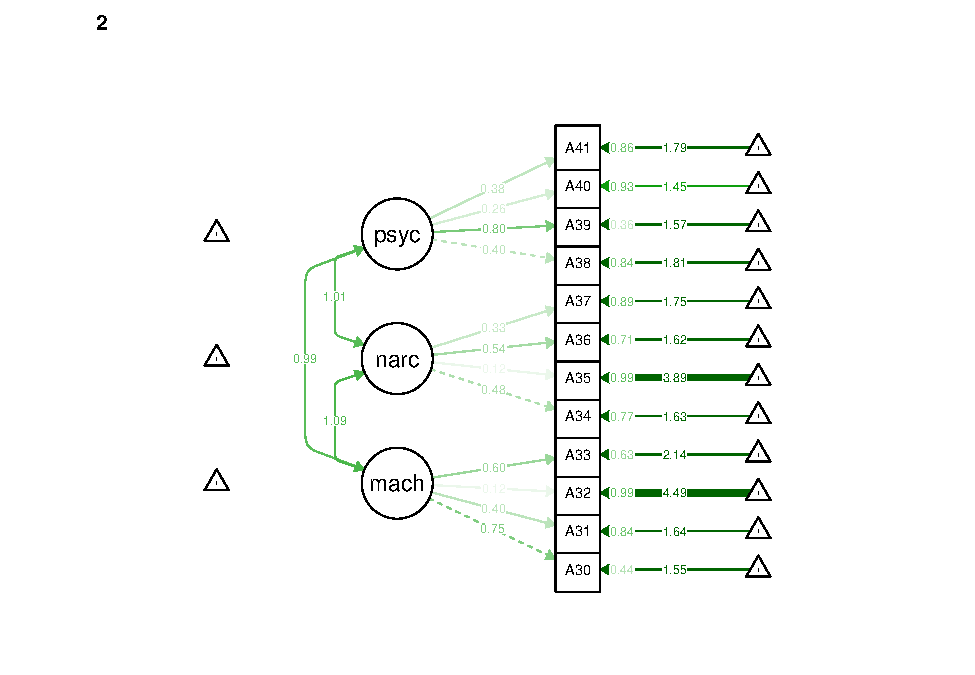
\includegraphics{SIOPpaper_files/figure-latex/measinv-2.pdf} 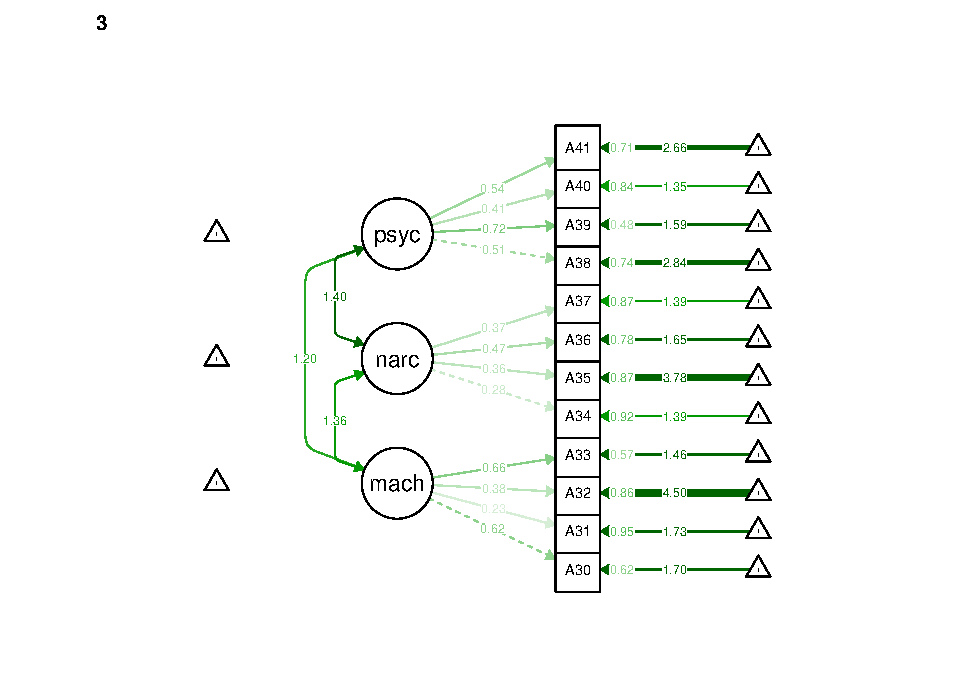
\includegraphics{SIOPpaper_files/figure-latex/measinv-3.pdf}

Yang also wanted correlations

\begin{lltable}

\begin{TableNotes}[para]
\normalsize{\textit{Note.} * p < 0.05; ** p < 0.01; *** p < 0.001}
\end{TableNotes}

\begin{longtable}{llllllllll}\noalign{\getlongtablewidth\global\LTcapwidth=\longtablewidth}
\caption{\label{tab:scalecors}Scale intercorrelations (all participants).}\\
\toprule
 & \multicolumn{1}{c}{1} & \multicolumn{1}{c}{2} & \multicolumn{1}{c}{3} & \multicolumn{1}{c}{4} & \multicolumn{1}{c}{5} & \multicolumn{1}{c}{6} & \multicolumn{1}{c}{7} & \multicolumn{1}{c}{$M$} & \multicolumn{1}{c}{$SD$}\\
\midrule
\endfirsthead
\caption*{\normalfont{Table \ref{tab:scalecors} continued}}\\
\toprule
 & \multicolumn{1}{c}{1} & \multicolumn{1}{c}{2} & \multicolumn{1}{c}{3} & \multicolumn{1}{c}{4} & \multicolumn{1}{c}{5} & \multicolumn{1}{c}{6} & \multicolumn{1}{c}{7} & \multicolumn{1}{c}{$M$} & \multicolumn{1}{c}{$SD$}\\
\midrule
\endhead
1. Machiavelliansm & - &  &  &  &  &  &  & 1.62 & 0.78\\
2. Narcissism & .29*** & - &  &  &  &  &  & 3.69 & 1.07\\
3. Psychopathy & .57*** & .19*** & - &  &  &  &  & 1.51 & 0.62\\
4. Fairness & -.34*** & -.02 & -.45*** & - &  &  &  & 5.40 & 0.84\\
5. GreedAvoidance & -.26*** & -.45*** & -.24*** & .27*** & - &  &  & 3.52 & 1.14\\
6. Modesty & -.23*** & -.43*** & -.17*** & .15** & .43*** & - &  & 3.72 & 0.85\\
7. Sincerity & -.14** & .04 & -.04 & .23*** & .11* & .18*** & - & 3.85 & 0.74\\
8. HonestyHumility & -.38*** & -.37*** & -.35*** & .61*** & .77*** & .68*** & .51*** & 4.12 & 0.59\\
\bottomrule
\addlinespace
\insertTableNotes
\end{longtable}

\end{lltable}

\begin{lltable}

\begin{TableNotes}[para]
\normalsize{\textit{Note.} * p < 0.05; ** p < 0.01; *** p < 0.001}
\end{TableNotes}

\begin{longtable}{llllllllll}\noalign{\getlongtablewidth\global\LTcapwidth=\longtablewidth}
\caption{\label{tab:scalecors}Scale intercorrelations (working adults low-stakes).}\\
\toprule
 & \multicolumn{1}{c}{1} & \multicolumn{1}{c}{2} & \multicolumn{1}{c}{3} & \multicolumn{1}{c}{4} & \multicolumn{1}{c}{5} & \multicolumn{1}{c}{6} & \multicolumn{1}{c}{7} & \multicolumn{1}{c}{$M$} & \multicolumn{1}{c}{$SD$}\\
\midrule
\endfirsthead
\caption*{\normalfont{Table \ref{tab:scalecors} continued}}\\
\toprule
 & \multicolumn{1}{c}{1} & \multicolumn{1}{c}{2} & \multicolumn{1}{c}{3} & \multicolumn{1}{c}{4} & \multicolumn{1}{c}{5} & \multicolumn{1}{c}{6} & \multicolumn{1}{c}{7} & \multicolumn{1}{c}{$M$} & \multicolumn{1}{c}{$SD$}\\
\midrule
\endhead
1. Machiavelliansm & - &  &  &  &  &  &  & 1.74 & 0.86\\
2. Narcissism & .31*** & - &  &  &  &  &  & 3.64 & 1.10\\
3. Psychopathy & .61*** & .20** & - &  &  &  &  & 1.73 & 0.74\\
4. Fairness & -.35*** & -.02 & -.45*** & - &  &  &  & 5.27 & 0.88\\
5. GreedAvoidance & -.27*** & -.45*** & -.21** & .30*** & - &  &  & 3.53 & 1.08\\
6. Modesty & -.18** & -.42*** & -.16* & .24*** & .43*** & - &  & 3.72 & 0.82\\
7. Sincerity & -.15* & .10 & -.08 & .26*** & .13 & .14* & - & 3.79 & 0.73\\
8. HonestyHumility & -.36*** & -.33*** & -.35*** & .68*** & .76*** & .68*** & .52*** & 4.08 & 0.59\\
\bottomrule
\addlinespace
\insertTableNotes
\end{longtable}

\end{lltable}

\begin{lltable}

\begin{TableNotes}[para]
\normalsize{\textit{Note.} * p < 0.05; ** p < 0.01; *** p < 0.001}
\end{TableNotes}

\begin{longtable}{llllllllll}\noalign{\getlongtablewidth\global\LTcapwidth=\longtablewidth}
\caption{\label{tab:scalecors}Scale intercorrelations (working adults high-stakes).}\\
\toprule
 & \multicolumn{1}{c}{1} & \multicolumn{1}{c}{2} & \multicolumn{1}{c}{3} & \multicolumn{1}{c}{4} & \multicolumn{1}{c}{5} & \multicolumn{1}{c}{6} & \multicolumn{1}{c}{7} & \multicolumn{1}{c}{$M$} & \multicolumn{1}{c}{$SD$}\\
\midrule
\endfirsthead
\caption*{\normalfont{Table \ref{tab:scalecors} continued}}\\
\toprule
 & \multicolumn{1}{c}{1} & \multicolumn{1}{c}{2} & \multicolumn{1}{c}{3} & \multicolumn{1}{c}{4} & \multicolumn{1}{c}{5} & \multicolumn{1}{c}{6} & \multicolumn{1}{c}{7} & \multicolumn{1}{c}{$M$} & \multicolumn{1}{c}{$SD$}\\
\midrule
\endhead
1. Machiavelliansm & - &  &  &  &  &  &  & 1.57 & 0.74\\
2. Narcissism & .29*** & - &  &  &  &  &  & 3.71 & 1.06\\
3. Psychopathy & .53*** & .21*** & - &  &  &  &  & 1.42 & 0.55\\
4. Fairness & -.33*** & -.03 & -.40*** & - &  &  &  & 5.54 & 0.78\\
5. GreedAvoidance & -.26*** & -.46*** & -.29*** & .24*** & - &  &  & 3.52 & 1.19\\
6. Modesty & -.27*** & -.43*** & -.18** & .06 & .42*** & - &  & 3.73 & 0.88\\
7. Sincerity & -.14* & -.02 & .02 & .17* & .09 & .21** & - & 3.90 & 0.74\\
8. HonestyHumility & -.39*** & -.41*** & -.34*** & .54*** & .78*** & .68*** & .50*** & 4.17 & 0.58\\
\bottomrule
\addlinespace
\insertTableNotes
\end{longtable}

\end{lltable}

\begin{lltable}

\begin{TableNotes}[para]
\normalsize{\textit{Note.} * p < 0.05; ** p < 0.01; *** p < 0.001}
\end{TableNotes}

\begin{longtable}{llllllllll}\noalign{\getlongtablewidth\global\LTcapwidth=\longtablewidth}
\caption{\label{tab:scalecors}Scale intercorrelations (students low-stakes).}\\
\toprule
 & \multicolumn{1}{c}{1} & \multicolumn{1}{c}{2} & \multicolumn{1}{c}{3} & \multicolumn{1}{c}{4} & \multicolumn{1}{c}{5} & \multicolumn{1}{c}{6} & \multicolumn{1}{c}{7} & \multicolumn{1}{c}{$M$} & \multicolumn{1}{c}{$SD$}\\
\midrule
\endfirsthead
\caption*{\normalfont{Table \ref{tab:scalecors} continued}}\\
\toprule
 & \multicolumn{1}{c}{1} & \multicolumn{1}{c}{2} & \multicolumn{1}{c}{3} & \multicolumn{1}{c}{4} & \multicolumn{1}{c}{5} & \multicolumn{1}{c}{6} & \multicolumn{1}{c}{7} & \multicolumn{1}{c}{$M$} & \multicolumn{1}{c}{$SD$}\\
\midrule
\endhead
1. Machiavelliansm & - &  &  &  &  &  &  & NA & NA\\
2. Narcissism & NA & - &  &  &  &  &  & NA & NA\\
3. Psychopathy & NA & NA & - &  &  &  &  & NA & NA\\
4. Fairness & NA & NA & NA & - &  &  &  & NA & NA\\
5. GreedAvoidance & NA & NA & NA & NA & - &  &  & NA & NA\\
6. Modesty & NA & NA & NA & NA & NA & - &  & NA & NA\\
7. Sincerity & NA & NA & NA & NA & NA & NA & - & NA & NA\\
8. HonestyHumility & NA & NA & NA & NA & NA & NA & NA & NA & NA\\
\bottomrule
\addlinespace
\insertTableNotes
\end{longtable}

\end{lltable}

\hypertarget{discussion}{%
\section{Discussion}\label{discussion}}

\newpage

\hypertarget{references}{%
\section{References}\label{references}}

\begingroup
\setlength{\parindent}{-0.5in}
\setlength{\leftskip}{0.5in}

\hypertarget{refs}{}
\begin{CSLReferences}{1}{0}
\leavevmode\hypertarget{ref-R-papaja}{}%
Aust, F., \& Barth, M. (2020). \emph{{papaja}: {Create} {APA} manuscripts with {R Markdown}}. Retrieved from \url{https://github.com/crsh/papaja}

\leavevmode\hypertarget{ref-church2011cross}{}%
Church, A. T., Alvarez, J. M., Mai, N. T., French, B. F., Katigbak, M. S., \& Ortiz, F. A. (2011). Are cross-cultural comparisons of personality profiles meaningful? Differential item and facet functioning in the revised NEO personality inventory. \emph{Journal of Personality and Social Psychology}, \emph{101}(5), 1068--1089.

\leavevmode\hypertarget{ref-itc_2017}{}%
Commission, I. T. (2017). The ITC guidelines for translating and adapting tests (second edition).

\leavevmode\hypertarget{ref-R-corx}{}%
Conigrave, J. (2020). \emph{Corx: Create and format correlation matrices}. Retrieved from \url{https://CRAN.R-project.org/package=corx}

\leavevmode\hypertarget{ref-geng2015dirty}{}%
Geng, Y., Sun, Q., Huang, J., Zhu, Y., \& Han, X. (2015). Dirty dozen and short dark triad: A chinese validation of two brief measures of the dark triad. \emph{Chinese Journal of Clinical Psychology}, \emph{23}(2), 246--250.

\leavevmode\hypertarget{ref-grigoras2020measurement}{}%
Grigoras, M., Butucescu, A., Miulescu, A., Opariuc-Dan, C., \& Iliescu, D. (2020). The measurement invariance of the short dark triad: Implications for high-and low-stakes contexts. \emph{Journal of Individual Differences}, 1--12.

\leavevmode\hypertarget{ref-jonason2010dirty}{}%
Jonason, P. K., \& Webster, G. D. (2010). The dirty dozen: A concise measure of the dark triad. \emph{Psychological Assessment}, \emph{22}(2), 420--432.

\leavevmode\hypertarget{ref-R-semTools}{}%
Jorgensen, T. D., Pornprasertmanit, S., Schoemann, A. M., \& Rosseel, Y. (2021). \emph{\texttt{semTools}: {U}seful tools for structural equation modeling}. Retrieved from \url{https://CRAN.R-project.org/package=semTools}

\leavevmode\hypertarget{ref-meredith1993measurement}{}%
Meredith, W. (1993). Measurement invariance, factor analysis and factorial invariance. \emph{Psychometrika}, \emph{58}(4), 525--543.

\leavevmode\hypertarget{ref-R-foreign}{}%
R Core Team. (2020). \emph{Foreign: Read data stored by 'minitab', 's', 'SAS', 'SPSS', 'stata', 'systat', 'weka', 'dBase', ...} Retrieved from \url{https://CRAN.R-project.org/package=foreign}

\leavevmode\hypertarget{ref-R-base}{}%
R Core Team. (2021). \emph{R: A language and environment for statistical computing}. Vienna, Austria: R Foundation for Statistical Computing. Retrieved from \url{https://www.R-project.org/}

\leavevmode\hypertarget{ref-R-lavaan}{}%
Rosseel, Y. (2012). {lavaan}: An {R} package for structural equation modeling. \emph{Journal of Statistical Software}, \emph{48}(2), 1--36. Retrieved from \url{https://www.jstatsoft.org/v48/i02/}

\leavevmode\hypertarget{ref-schmitt2008measurement}{}%
Schmitt, N., \& Kuljanin, G. (2008). Measurement invariance: Review of practice and implications. \emph{Human Resource Management Review}, \emph{18}(4), 210--222.

\leavevmode\hypertarget{ref-vandevelopmetrics}{}%
Schoot, R. van de, Lugtig, P., \& Hox, J. (2012). Developmetrics: A checklist for testing measurement invariance. \emph{European Journal of Developmental Psychology}, \emph{9}(4), 486--492.

\leavevmode\hypertarget{ref-steinmetz2009testing}{}%
Steinmetz, H., Schmidt, P., Tina-Booh, A., Wieczorek, S., \& Schwartz, S. H. (2009). Testing measurement invariance using multigroup CFA: Differences between educational groups in human values measurement. \emph{Quality \& Quantity}, \emph{43}(4), 599--616.

\leavevmode\hypertarget{ref-R-careless}{}%
Yentes, R. D., \& Wilhelm, F. (2021). \emph{Careless: Procedures for computing indices of careless responding}.

\end{CSLReferences}

\endgroup


\end{document}
